\documentclass{article}
\usepackage[utf8]{inputenc}
\usepackage[hidelinks]{hyperref}
\usepackage{graphicx}
\usepackage{float}
\usepackage{caption}
\usepackage{subcaption}
\usepackage{biblatex} %Imports biblatex package
\usepackage{hyperref}
\hypersetup{colorlinks,linkcolor={blue},citecolor={blue},urlcolor={black}}  
\addbibresource{refs.bib} %Import the bibliography file

\newcommand{\todo}[1]{\textcolor{red}{[\textcolor{blue}{TODO:} #1]}}
\newcommand{\deep}[1]{\textcolor{cyan}{[Arnav Tuli: #1]}}
\newcommand{\pranjal}[1]{\textcolor{magenta}{[Deepanshu: #1]}}

\title{\textbf{Assignment-1 Submission}}
\author{\textbf{Indian Institute  of Technology Delhi}}
\date{\textbf{Software Rasterization}}




\begin{document}

\maketitle
\textbf{Name: Arnav Tuli\quad \quad Entry Number: 2019CS10424}\\
\textbf{Name: Deepanshu\quad Entry Number: 2019CS50427}
\maketitle

\section{Example: e1.cpp}

\section{Example: e2.cpp}
\section{Example: e3.cpp}
\section{Example: e4.cpp}
\section{Example: e5.cpp}

\section{Clock rasterization}
% code to add a figure that does not overflow the page
\begin{figure}[H]
    \centering
    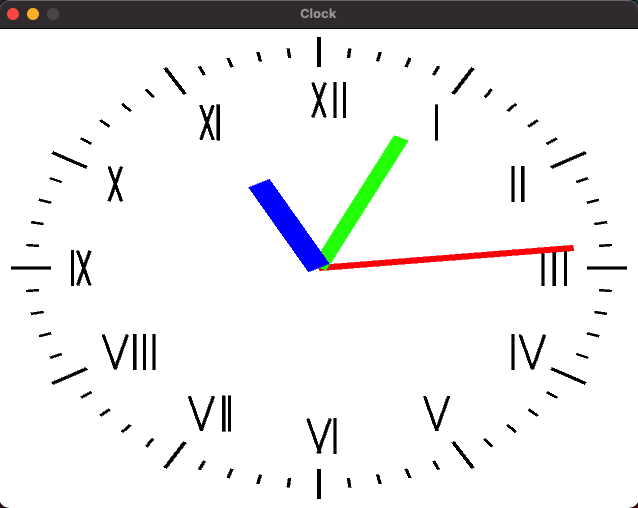
\includegraphics[width=.8\textwidth]{clock.png}
    \end{figure}

\section{3D scene rasterization}

\end{document}